%!TEX root = ../rapport.tex
%!TEX encoding = UTF-8 Unicode

% Chapitres "Introduction"

% modifié par Francis Valois, Université Laval
% 31/01/2011 - version 1.0 - Création du document

\chapter{Diagrammes de séquences}
\label{s:sequences}
Ce chapitre présente les différentes figures associées au diagramme des séquences. Ce diagramme est séparé selon quatre portions relatives aux fonctions particulières du robot. La figure \ref{fig:diagSeq1Ite1} présente les liens entre l'utilisateur et la kinocto. La figure \ref{diagSeq2Ite1} présente les liens entre la kinocto et son environnement afin de déterminer sa position. La figure \ref{diagSeq3Ite1} présente les liens entre la kinocto et la station de base pour la transmission et l'affichage de la trajectoire optimale. La lecture et la résolution du sudocube  y est aussi présenté. La figure \ref{diagSeq4Ite1} présente les liens entre la kinocto et ses différents périphériques lors de la production du dessin et de la confirmation de la résolution de la tâche.
\begin{figure}[htb]
\centering
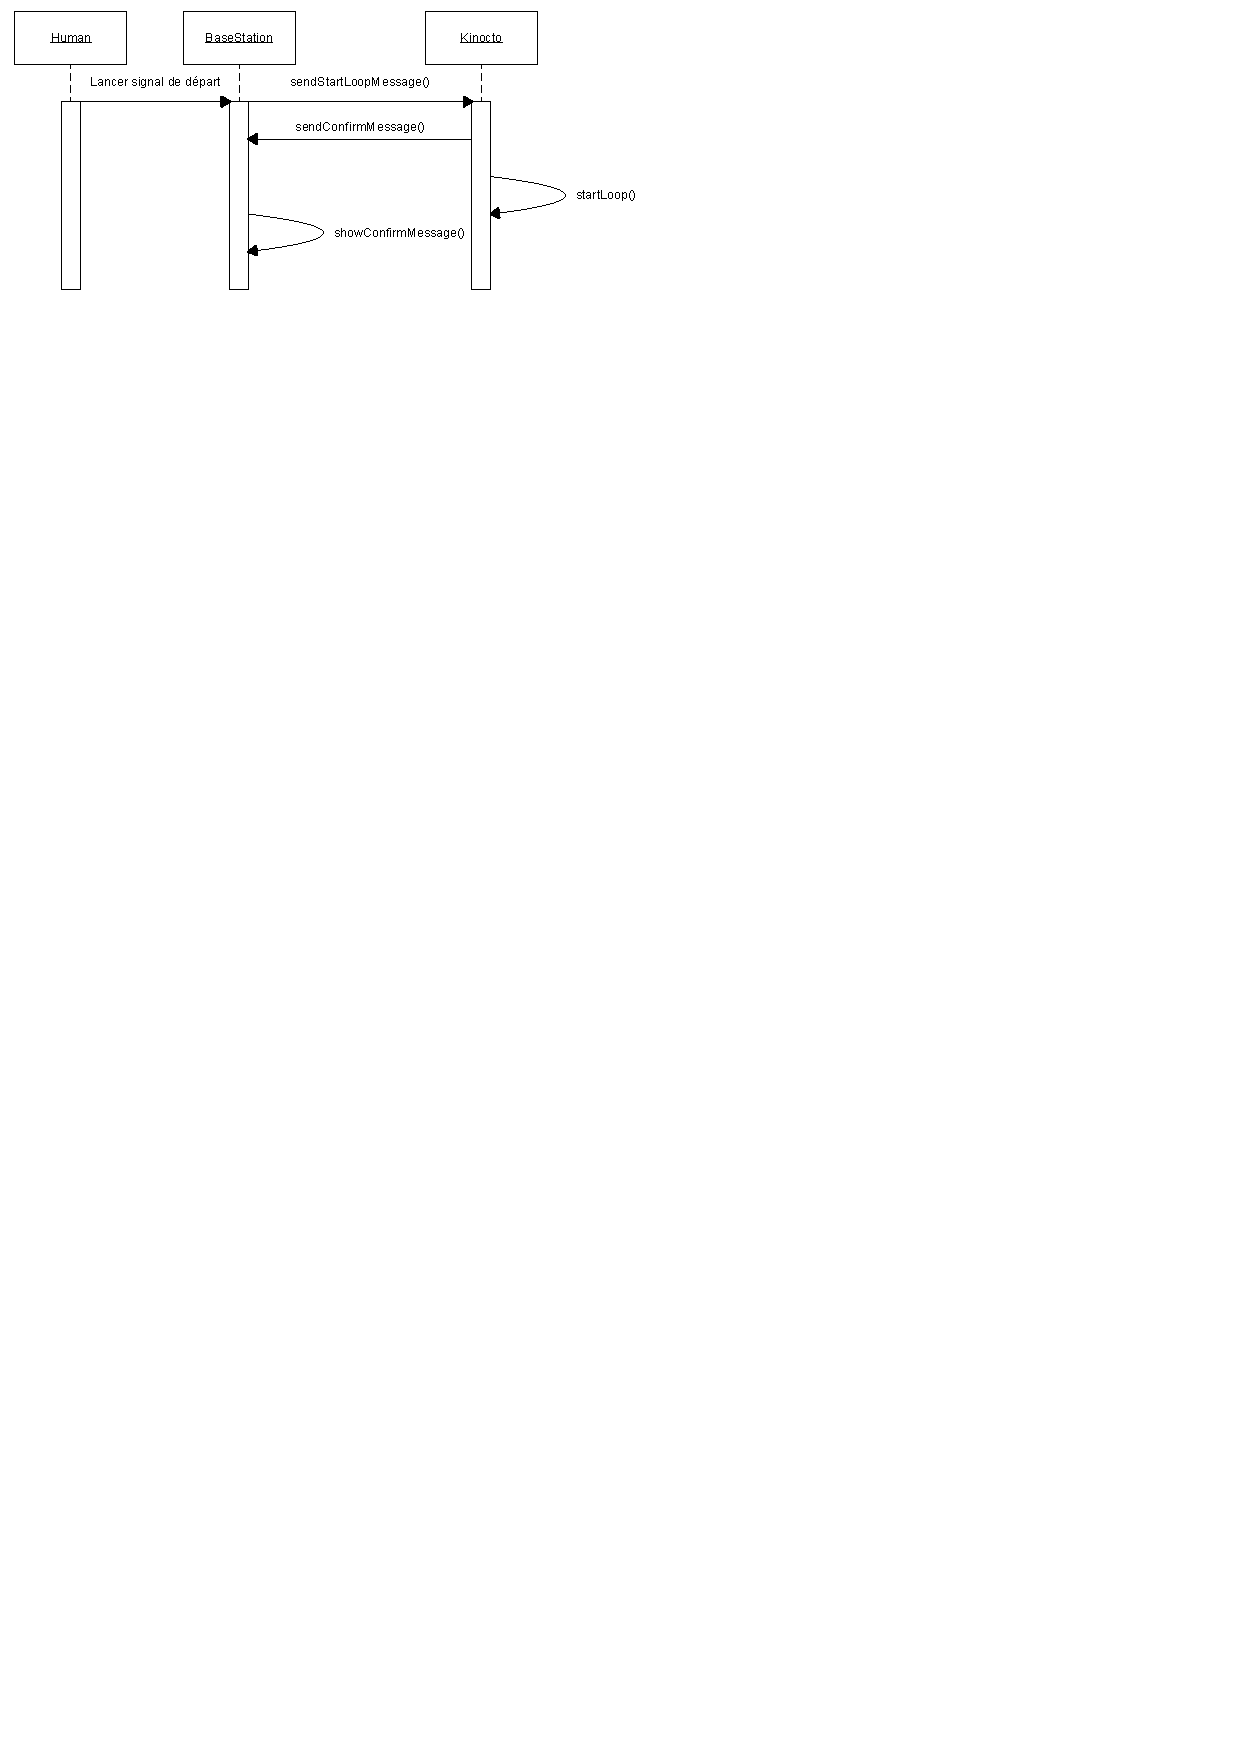
\includegraphics[scale=1]{fig/diagrammes_sequence1.pdf}
\caption{Diagramme des séquences présentant les liens entre l'utilisateur et la kinocto}
\label{fig:diagSeq1Ite1} 
\end{figure}
\begin{figure}[htb]
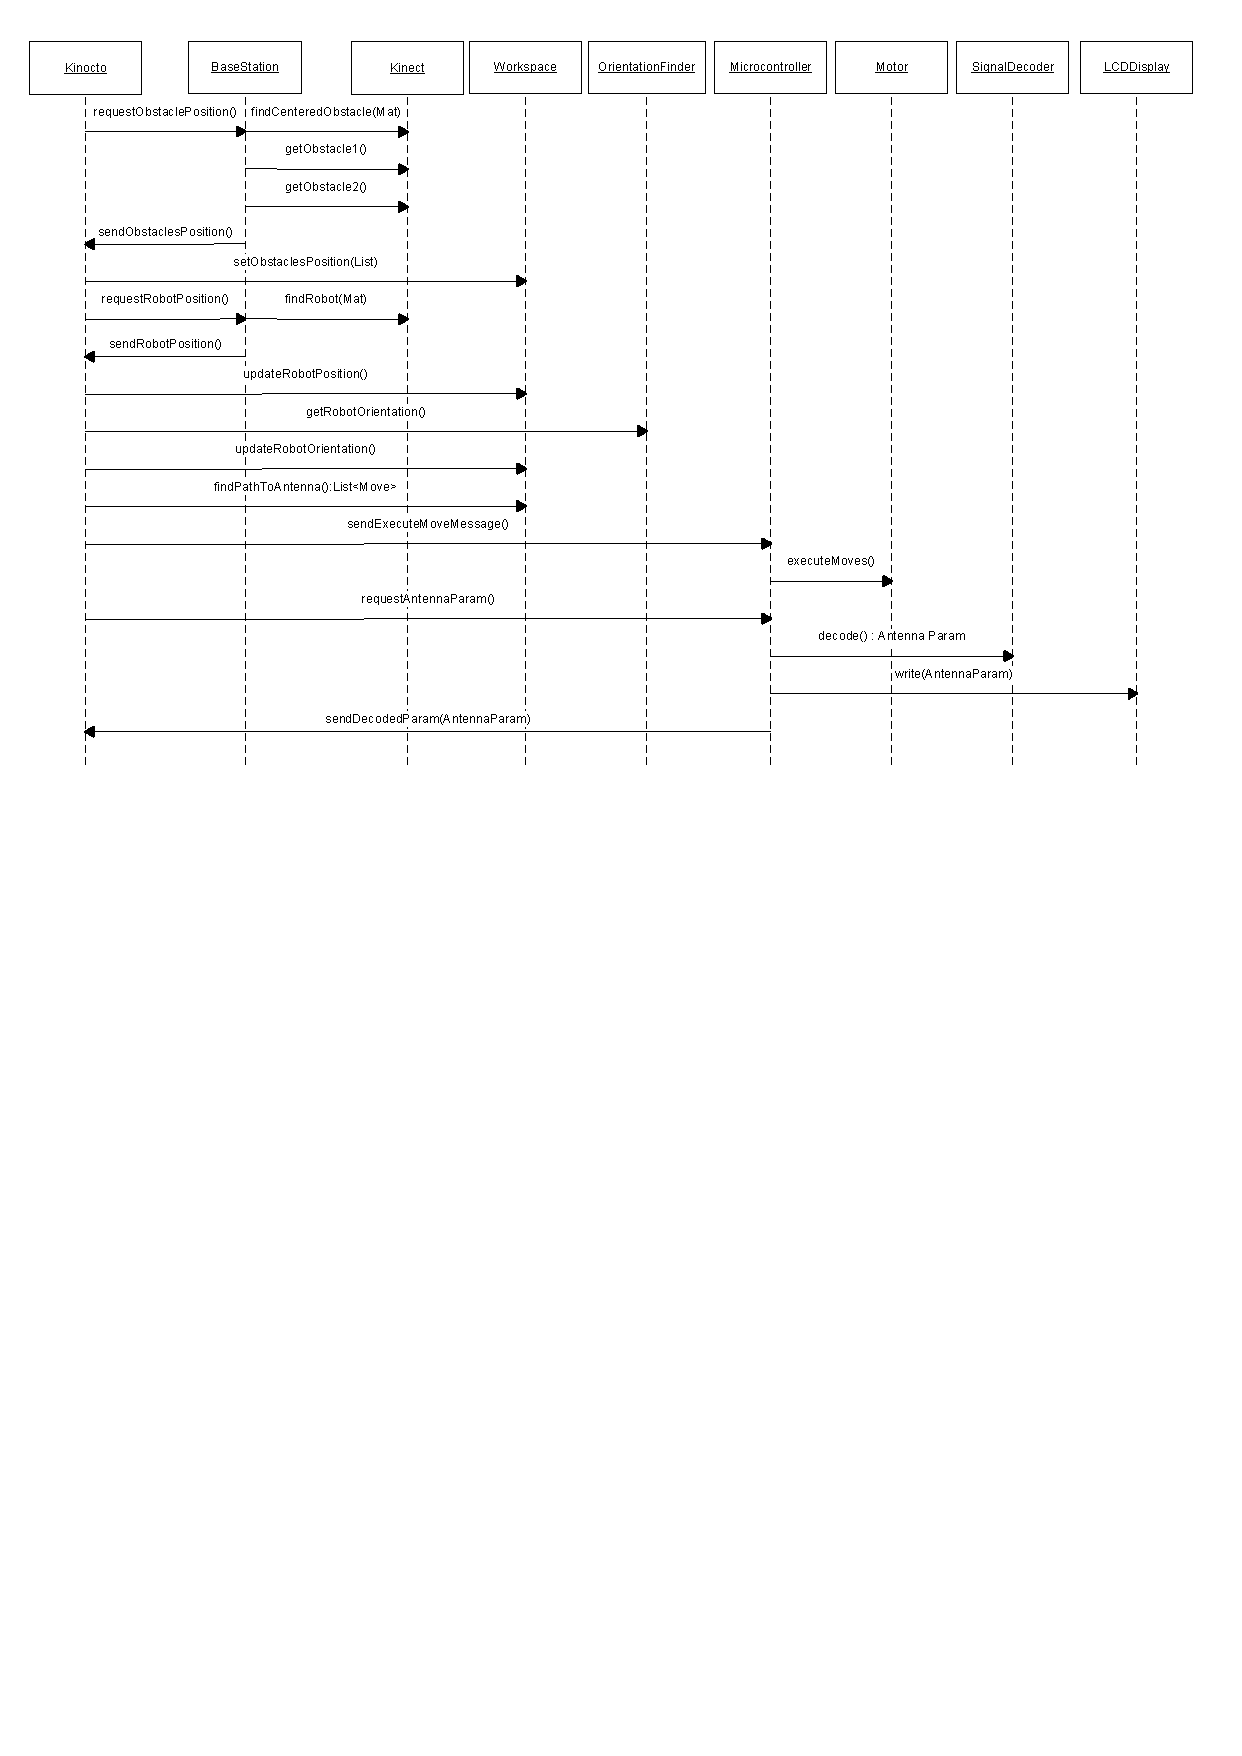
\includegraphics[scale=0.9]{fig/diagrammes_sequence2.pdf}
\caption{Diagramme des séquences présentant les liens entre la kinocto et son environnement afin de déterminer sa position}
\label{diagSeq2Ite1}
\end{figure}
\begin{figure}[htb]
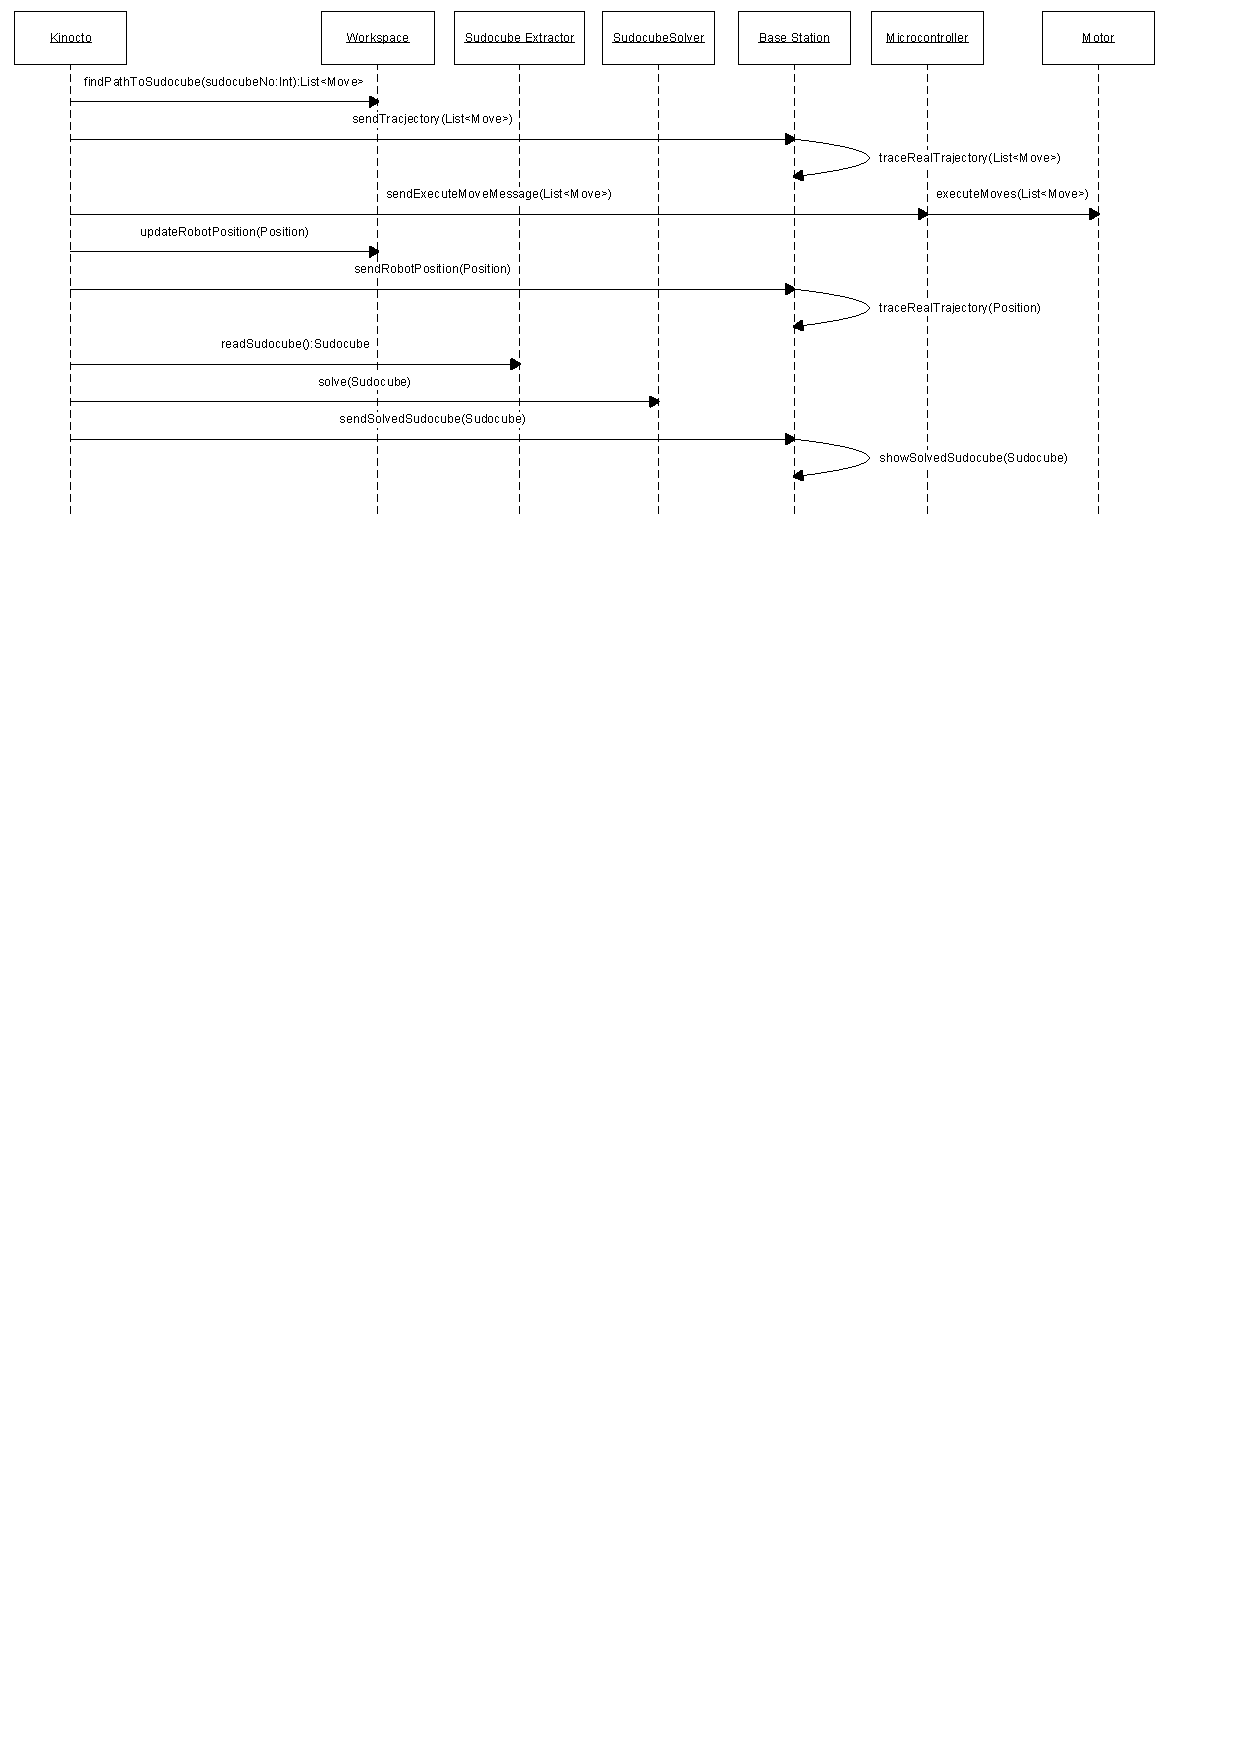
\includegraphics[scale=0.9]{fig/diagrammes_sequence3.pdf}
\caption{Diagramme des séquences présentant les liens entre la kinocto et la station de base pour la transmission et l'affichage de la trajectoire optimale vers la zone de lecture du sudocube, ainsi que la résolution de celui-ci}
\label{diagSeq3Ite1}
\end{figure}
\begin{figure}[htb]
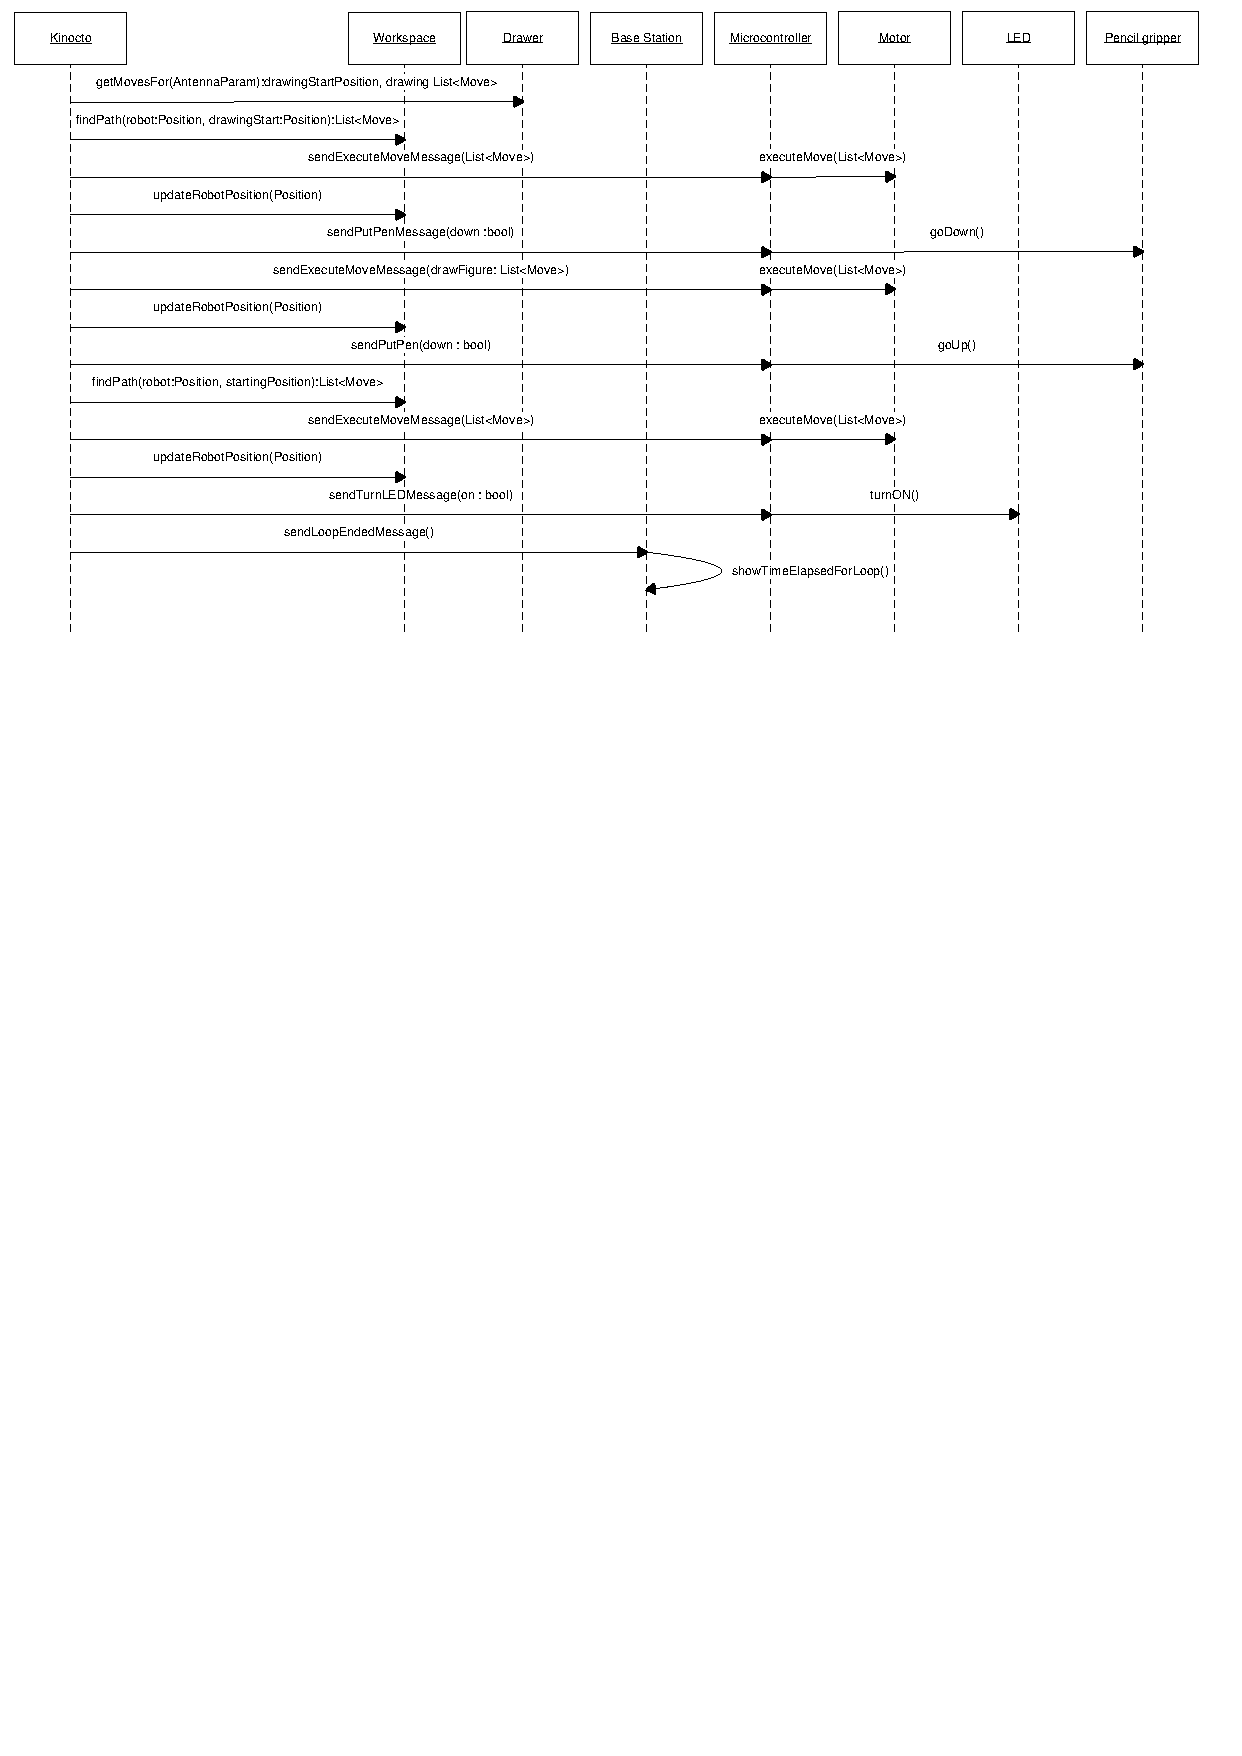
\includegraphics[scale=0.9]{fig/diagrammes_sequence4.pdf}
\caption{Diagramme des séquences présentant les liens entre la kinocto et ses différents périphériques lors de la production du dessin et de la confirmation de la résolution de la tâche}
\label{diagSeq4Ite1}
\end{figure}